\subsection{Methodology}


We propose a methodology to demystify GPU microarchitecture features and correlate them with programs' performance.
The workflow in figure~\ref{fig:workflow} consists of three major components: an instruction encoding\jli{replaced decoding} solver, a GPU assembler, and meticulous benchmarking.
%and two program sets: sample programs and microbenchmark.
% a deliberate microbenchmark
A sample program in figure~\ref{fig:workflow} is a synthetic PTX file which generates specific instructions as the input of the instruction solver.
Deliberate microbenchmarks are designed for our assembler to tune code at assembly language level and to help figure out the correlation between microarchitecture and performance.
%We dissemble a binary library (such as cuBLAS) to provide a high coverage of instructions to instruction solver.
%We use cuBLAS in this work since it contains nearly all needed instructions for SGEMM routine.

We first leverage CUDA binary tools ({\tt cuobjdump} or {\tt nvdiasm}) to disassemble {\tt cubin} generated by sample programs. % and the library.
% A library might provide a high coverage of instruction sets.
As introduced in section~\ref{sec:cuda}, generated assembly files ({\em sass}) provide instruction encodings to be cracked.
Our instruction solver takes the assembly files as the input to decode each field of 64-bit instructions.
We design a set of algorithms to solve all fields of a binary instruction, which include different types of {\em operands}, {\em opcodes}, and {\em modifiers}.
%The solver uncovers some undocumented ISA specifications,
%which is used to implement an naive assembler.
Our assembler translates every instruction field to get $64$-bit binaries and then encapsulates them with an ELF header to generate an executable cubin file.
% which can be used by CUDA driver APIs.
In the benchmarking workflow (red arrows in figure~\ref{fig:workflow}), microbenchmarks are tuned at the assembly language level using our assembler.
GPU microarchitecture features are explored during benchmarking, which will guide the optimization of real programs.
% In the end, the tuning process will lead to some practical observations on the correlation between microarchitecture and performance.


\begin{figure}[htbp]
\begin{center}
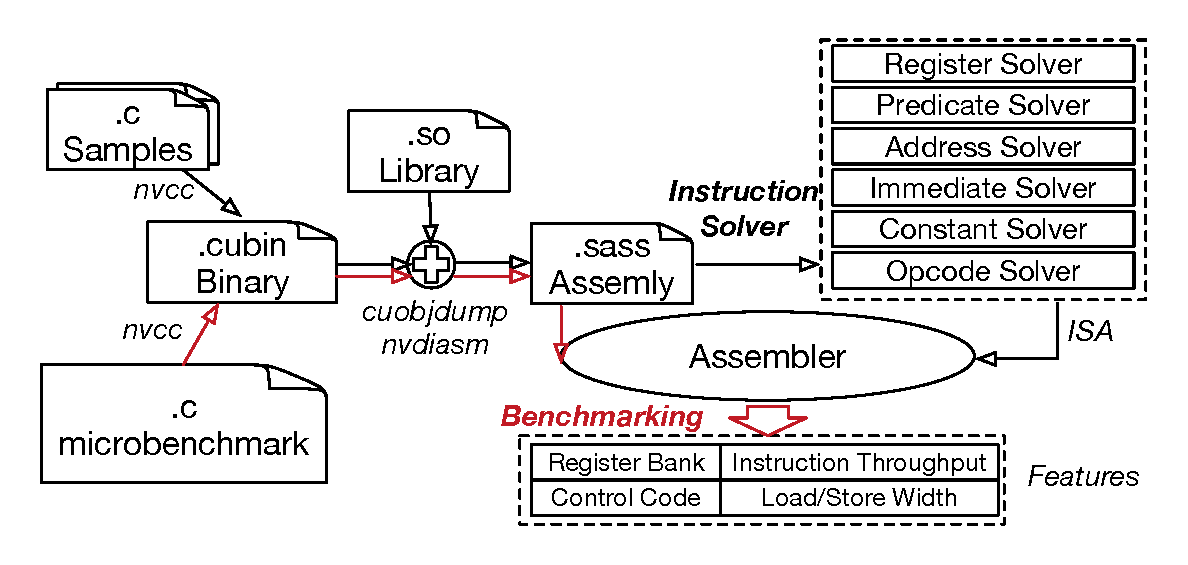
\includegraphics[scale=0.45]{methodology}
\caption{A schematic diagram of demystifying GPU microarchitecture features by leveraging CUDA binary tools. The black arrows
represent the workflow of instruction solver while the red ones represents benchmarking to find out the correlation between microarchitecture and performance.\jli{microbenchmark->microbenchmarks, .c->.cu}}
\label{fig:workflow}
\end{center}
\end{figure}
